\documentclass[pdflatex,compress]{beamer}

%\usetheme[dark,framenumber,totalframenumber]{ElektroITK}
\usetheme[darktitle,framenumber,totalframenumber]{ElektroITK}

\renewcommand{\figurename}{Gambar} \setbeamertemplate{caption}[numbered]

\usepackage{graphicx}
\usepackage{multicol}

\title{FORENSIKA SUARA}
\subtitle{Sejarah Audio Forensik}

\author{Tim Dosen Pengampu}

\begin{document}

\maketitle

\section{Pengantar}

\begin{frame}{Pengantar}
	\begin{itemize}
		\item Audio forensik bergantung pada ketersediaan rekaman audio.
		\item Rekaman audio diambil di luar studio rekaman.
		\item Diambil secara rahasia/ penyadapan. Melanggar HAM?
		\item Kerancuan identitas dari suara yang direkam dengan kualitas suara yang buruk.
		\item Rekaman palsu/ editan?
	\end{itemize}
\end{frame}

\section{McKeever Case}

\begin{frame}
	\frametitle{McKeever Case}
	\begin{itemize}
		\item Dua terdakwa: Thomas McKeever dan Lawrence Morrison (International Longshoremen's Association).
		\item Kasus pemerasan terhadap James J. Ball \& Sons
		\item Audio rekaman bukan berasal dari pemerintah, tapi dari terdakwa sendiri, Thomas McKeever.
		\item Setelah surat dakwaan dikeluarkan, Thomas McKeever melakukan perekaman percakapan dengan George Ball.
		\item Kesaksian yang tidak konsisten.
		\item Di pengadilan, hakim meminta G. Ball untuk mendengarkan suara rekaman, tapi tidak untuk juri. Dan membenarkan rekaman tersebut.
	\end{itemize}
\end{frame}

\begin{frame}{McKeever Case}
	\begin{itemize}
		\item Pembela minta juri untuk mendengarkan juga. Menegaskan ketidakkonsistenan.
		\item Pembela keberatan. Pembela tidak memiliki dasar yang kuat.
		\item \textit{"untuk keakuratan atau keaslian rekaman kaset. Tidak ada bukti saat ini di depan Pengadilan bahwa rekaman yang dibuat oleh para terdakwa adalah rekaman dari percakapan apapun antara McKeever dan George Ball."}
		\item Keputusan pengadilan menolak audio rekaman dimainkan di pengadilan berdasarkan \textbf{7 prinsip autentikasi audio}
	\end{itemize}
\end{frame}

\begin{frame}
\frametitle{Seven Tenets of Audio Authenticity}
	\begin{itemize}
		\item 	A review of the authorities leads to the conclusion that, before a sound recording is admitted into evidence, a foundation must be established by showing the following facts:
		\begin{enumerate}
			\item That the recording device was capable of taking the conversation now offered in evidence.
			\item That the operator of the device was competent to operate the device.
			\item That the recording is authentic and correct.
			\item That changes, additions, or deletions have not been made in the recording.
			\item That the recording has been preserved in a manner that is shown to the court.
			\item That the speakers are identified.
			\item That the conversation elicited was made voluntarily and in good faith, without any kind of inducement.
		\end{enumerate}
	\end{itemize}
\end{frame}

\section{MacMillan Case}

\begin{frame}
	\frametitle{MacMillan Case}
	\begin{itemize}
		\item Kasus transaksi narkotika tahun 1974
		\item Informan: Beverly Johnson $\leftarrow$ menggunakan alat perekam di telpon.
		\item Harold McMillan terlibat perencanaan pembelian heroin.
		\item Di persidangan, hakim mengizinkan penuntut untuk memainkan audio rekaman dan juga membaca transkrip rekaman.
		\item Pembela keberatan, penuntut belum menetapkan otentisitas dan landasan hukum.
	\end{itemize}
\end{frame}

\section{Prosedur FBI}

\begin{frame}
	\frametitle{Prosedur FBI}
	\begin{itemize}
		\item Pengembangan dari 7 tenets pada kasus McKeever menjadi 12 tenets.
		\begin{enumerate}
			\item Evidence marking.
			\item Physical inspection.
			\item Recorded track position and configuration.
			\item Azimuth alignment determination.
			\item Playback speed analysis.
			\item Proper playback setup.
			\item Overall aural review.
			\item Overall FFT review.
			\item Setup of enhancement devices.
			\item Copying process.
			\item Work notes.
			\item Reporting.
		\end{enumerate}
	\end{itemize}
\end{frame}

\section{Identifikasi Pembicara dan Voice Prints}

\begin{frame}
	\frametitle{Identifikasi Pembicara \\dan Voice Prints}
	\begin{itemize}
		\item Istilah \textit{Voiceprint} pertama kali oleh Bell Telephone Laboratories tahun 1944.
		\item Dimensi oral pembicara, pharyngeal dan nasal cavity $\rightarrow$ menentukan keunikan spectrogram $\rightarrow$ identifikasi pembicara
		\item Tahun 1960 - 1970, metode aural-spectrographic $\rightarrow$ membandingkan spectrogram pembicara yang tidak diketahui terhadap serangkaian spectrogram yang pembicara yang diketahui.
		\item Membandingkan antara pendengaran + penglihatan (pengamatan spectrogram)
	\end{itemize}
\end{frame}

\begin{frame}{Identifikasi Pembicara \\dan Voice Prints}
	\begin{itemize}
		\item Menghasilkan 5 opini yang mungkin
		\begin{enumerate}
			\item Positive identification (the suspect’s speech positively matches the unknown
			recorded speech).
			\item Probable identification.
			\item No decision.
			\item Probable elimination.
			\item Positive elimination.
		\end{enumerate}
	\end{itemize}
\end{frame}

\section{Digital Forensic Analyst Team (DFAT)}

\begin{frame}
	\frametitle{Digital Forensic Analyst Team\\(DFAT)}
	\begin{itemize}
		\item Semakin banyak penggunaan teknologi $\rightarrow$ barang bukti digital semakin banyak.
		\item Puslabform Bareskrim Polri (Pusat Laboratorium Forensik) membentuk Digital Forensic Analyst Team (DFAT) pada tanggal 18 Januari 2010
		\item DFAT berada di bawah Departmen Fisika dan Komputer Forensik.
	\end{itemize}
\end{frame}

\begin{frame}{Digital Forensic Analyst Team\\(DFAT)}
	\begin{center}
		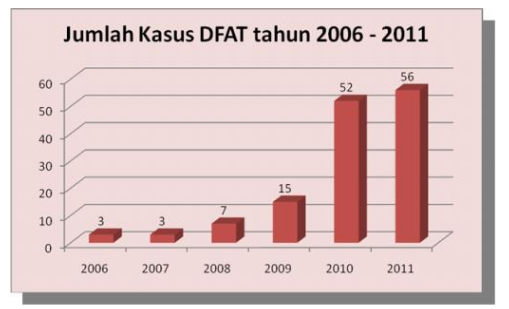
\includegraphics[width=0.7\linewidth]{img/img01}
	\end{center}
\end{frame}

\begin{frame}{Digital Forensic Analyst Team\\(DFAT)}
	\begin{center}
		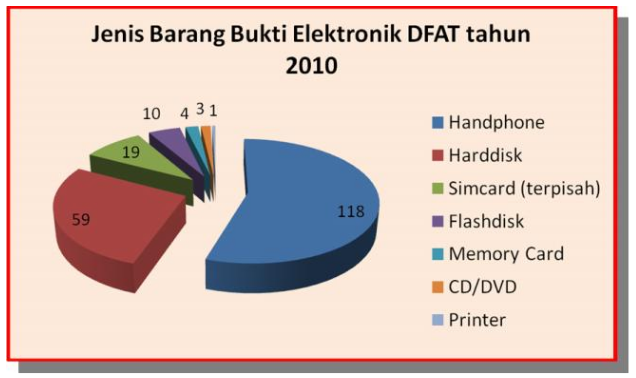
\includegraphics[width=0.7\linewidth]{img/img02}
	\end{center}
\end{frame}

\begin{frame}{Digital Forensic Analyst Team\\(DFAT)}
	\begin{center}
		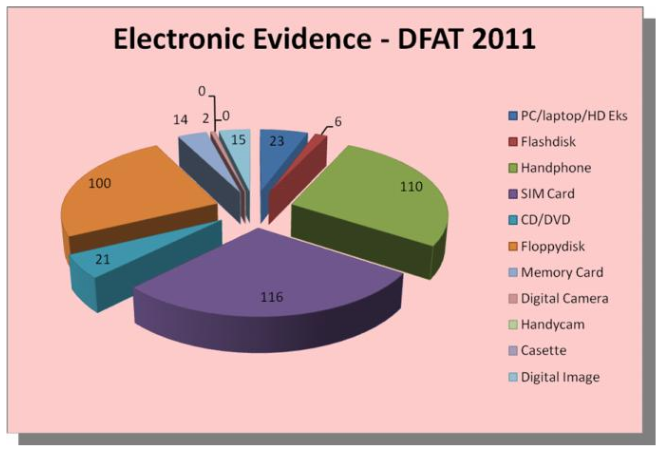
\includegraphics[width=0.7\linewidth]{img/img03}
	\end{center}
\end{frame}

\section{Komisi Pemberantasan Korupsi (KPK)}

\begin{frame}
	\frametitle{Komisi Pemberantasan Korupsi\\(KPK)}
	\begin{itemize}
		\item KPK + Ahli Forensik
		\begin{itemize}
			\item Laboratorium Akusik ITB
			\item Laboratorium Akustik ITS (VibrasticLab)
		\end{itemize}
		\item ITB: Analisis pitch dan formant
		\item ITS: Analisis itakura-saito distance
	\end{itemize}
	\begin{center}
		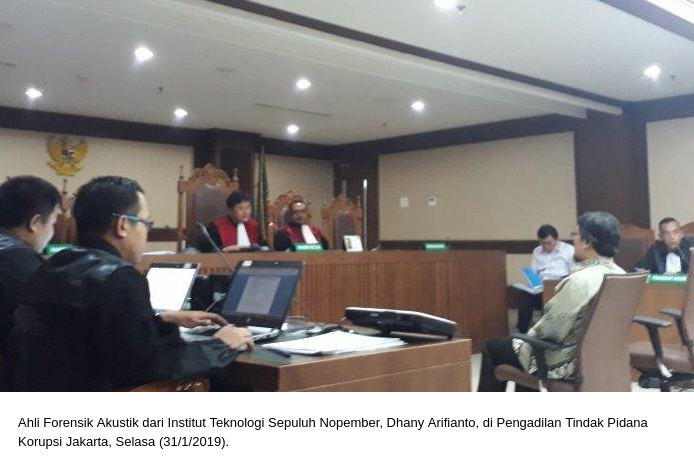
\includegraphics[width=0.5\linewidth]{img/img04}
	\end{center}
\end{frame}

\section{Referensi}

\begin{frame}
	\frametitle{Referensi}
	\begin{enumerate}
		\item Maher, R.C., (2018). Principles of Forensic Audio Analysis. New York: Springer.
		\item Al-Azhar, M. N. (2011). Audio Forensic: Theory And Analysis. Jakarta: Pusat Laboratorium Forensik Polri
		Bidang Fisika Dan Komputer Forensik.
		\item https://www.tribunnews.com/nasional/2019/01/31/ahli-forensik-akustik-tidak-bisa-memastikan-originalitas-rekaman-penyidik-kpk
	\end{enumerate}
\end{frame}

\end{document}
